\documentclass[12pt]{article}

\usepackage{sbc-template}

\usepackage{graphicx,url}

%\usepackage[brazil]{babel}
\usepackage[latin1]{inputenc}


\sloppy

\title{Uma an�lise de pad�es em senhas}

\author{Marino Souza S., Nilton V. C. J�nior, Luiz R. Rios}

\address{Instituto de Matem�tica -- Universidade Federal da Bahia
(UFBA)\\
\email{\{marino, niltonvasques\}@openmailbox.org, luizromario@gmail.com}
}

\begin{document}

\maketitle

\begin{resumo}
O m�todo de adivinha��o de senhas por for�a bruta necessita de um bom dicion�rio a fim de conseguir o maior n�mero de advinha��es poss�veis. Motivando-se no trabalho de \cite{chinas}. O presente artigo visa executar uma an�lise em cima de senhas web com o objetivo de encontrar padr�es que futuramente sirvam para melhorar dicion�rio de adivinha��o, ou desenvolver melhores pol�ticas de senhas.
\end{resumo}


\section{Introdu��o}

As bases de senhas utilizadas neste trabalho foram encontradas em sua maior parte no website SkullSecurity (https://blog.skullsecurity.org/) contendo senhas de provavel usu�rios de lingua inglesa, e outra base encontrada no PasteBin contendo um org�o de defesa de um governo de um pa�s que neste trabalho ser� omitido o nome, algumas vezes utilizado o codnome: BrArmy.
A quantidade de senhas totalizaram 64,493 provindas do SkullSecurity e 7,834 do BrArmy. Em ambos as bases de senhas haviam senhas em branco e com charset inv�lido que podem afetar as an�lises. Ap�s a filtragem de alguns desses dados a quantidade total caiu para 64,463 da SkullSecurity e 7,833 da BrArmy.
Durante este trabalho os autores preferiam utilizar o sistema internacional para representa��o de n�meros reais e multiplos de mil.

\section{Estat�sticas Comuns} \label{sec:firstpage}

fazer uma explica��o da sess�o.

\begin{table}[ht]
    \centering

    \begin{tabular}{clr}
        \hline
        & Skull leak & BR army\\
        \hline
        1 & 123456(0.202\%) & 12345678(4.864\%)\\
        2 & password1(0.119\%) & 123456789(1.009\%) \\
        3 & fuck(0.092\%) & 87654321(0.230\%)\\
        4 & abc123(0.090\%) & 10203040(0.204\%)\\
        5 & fuckyou(0.064\%) & 06121966(0.153\%)\\
        \hline
    \end{tabular}

    \caption{Senhas mais usadas nas duas bases}
    \label{table:tablegeneral}

\end{table}

Explicar oq a tabela \ref{table:tablegeneral} significa.
%B�nh H�a Massacre, Guerra do vietnam 6 de dezembro de 1966

The abstract and ``resumo'' (if is the case) must be in 12 point Times font,
indented 0.8cm on both sides. The word \textbf{Abstract} and \textbf{Resumo},
should be written in boldface and must precede the text.

\subsection{Subsections}

The subsection titles must be in boldface, 12pt, flush left.

\begin{table}[h]
    \centering

    \begin{tabular}{r r r r r}
        \hline
        & Exatamente Oito Digitos & DDMMYYYY & MMDDYYYY & YYYYMMDD\\
        \hline
        Skull-leak & 638(0.990\%) & 25.547\% & 5.799\% & 2.978\%\\
        \hline
        BrArmy & 3,565(45.513\%) & 26.928\% & 10.659\% & 0.701\%\\
        \hline
    \end{tabular}

    \caption{texto da tabela}
    \label{table:table-date-eight}

\end{table}


\begin{table}[h]
    \centering

    \begin{tabular}{r r r r r}
        \hline
        & Exatamente Seis D�gitos & DDMMYY & MMDDYY & YYMMDD\\
        \hline
        Skull-leak & 1,066(1.654\%) & 36.210\% & 19.325\% & 11.445\%\\
        \hline
        BrArmy & 0\% & & & \\
        \hline
    \end{tabular}

    \caption{texto da tabela}
    \label{table:table-date-six}

\end{table}

\begin{table}[!h]
    \centering

    \begin{tabular}{clr}
        \hline
        & Skull leak & BR army\\
        \hline
        1 & password1(0.119\%) & flamengo(0.115\%)\\
        2 & fuck(0.092\%) & exercito(0.115\%) \\
        3 & fuckyou(0.064\%) & infantaria(0.115\%)\\
        4 & monkey(0.045\%) & cavalaria(0.102\%)\\
        5 & iloveyou1(0.043\%) & guilherme(0.077\%)\\
        \hline
    \end{tabular}

    \caption{Palavras Inglesas/Portuguesas mais usadas}
    \label{table:most-comon-language}

\end{table}

Curiosamente os usu�rio de lingua inglesa preferem senhas relacionadas a palavras de baixo cal�o, como apresentado em \ref{table:most-comon-language}, enquanto os usu�rio da base BrArmy recorrem em sua maioria a palavras que tem alguma rela��o as for�as armadas.


\section{Figures and Captions}\label{sec:figs}


Figure and table captions should be centered if less than one line
(Figure~1), otherwise justified and indented by 0.8cm on
both margins, as shown in Figure~2. The caption font must
be Helvetica, 10 point, boldface, with 6 points of space before and after each
caption.

% \begin{figure}[ht]
% \centering
% 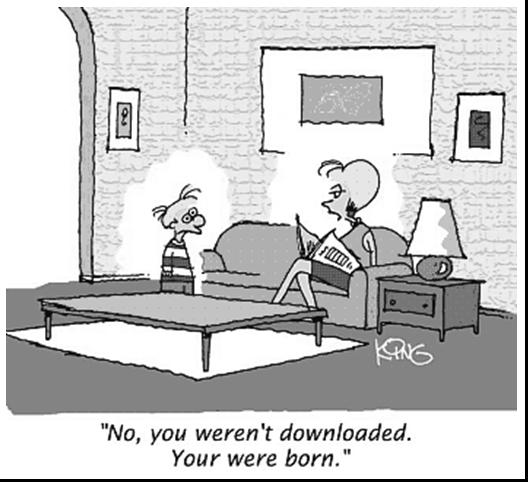
\includegraphics[width=.5\textwidth]{fig1.jpg}
% \caption{A typical figure}
% \label{fig:exampleFig1}
% \end{figure}

In tables, try to avoid the use of colored or shaded backgrounds, and avoid
thick, doubled, or unnecessary framing lines. When reporting empirical data,
do not use more decimal digits than warranted by their precision and
reproducibility. Table caption must be placed before the table (see Table 1)
and the font used must also be Helvetica, 10 point, boldface, with 6 points of
space before and after each caption.

\section{References}

Bibliographic references must be unambiguous and uniform.  We recommend giving
the author names references in brackets, e.g. \cite{chinas}.

\bibliographystyle{sbc}
\bibliography{referencias}

\end{document}
